%%
%% This is file `example.tex',
%% generated with the docstrip utility.
%%
%% The original source files were:
%%
%% coppe.dtx  (with options: `example')
%% 
%% This is a sample monograph which illustrates the use of `coppe' document
%% class and `coppe-unsrt' BibTeX style.
%% 
%% \CheckSum{1416}
%% \CharacterTable
%%  {Upper-case    \A\B\C\D\E\F\G\H\I\J\K\L\M\N\O\P\Q\R\S\T\U\V\W\X\Y\Z
%%   Lower-case    \a\b\c\d\e\f\g\h\i\j\k\l\m\n\o\p\q\r\s\t\u\v\w\x\y\z
%%   Digits        \0\1\2\3\4\5\6\7\8\9
%%   Exclamation   \!     Double quote  \"     Hash (number) \#
%%   Dollar        \$     Percent       \%     Ampersand     \&
%%   Acute accent  \'     Left paren    \(     Right paren   \)
%%   Asterisk      \*     Plus          \+     Comma         \,
%%   Minus         \-     Point         \.     Solidus       \/
%%   Colon         \:     Semicolon     \;     Less than     \<
%%   Equals        \=     Greater than  \>     Question mark \?
%%   Commercial at \@     Left bracket  \[     Backslash     \\
%%   Right bracket \]     Circumflex    \^     Underscore    \_
%%   Grave accent  \`     Left brace    \{     Vertical bar  \|
%%   Right brace   \}     Tilde         \~}
%%
\documentclass[grad,numbers]{coppe}
\usepackage{amsmath,amssymb}
\usepackage{hyperref}
\usepackage[utf8]{inputenc}
\usepackage[brazil]{babel}
\usepackage[T1]{fontenc}
\usepackage{graphicx}
\usepackage{amsmath}

\makelosymbols
\makeloabbreviations

\begin{document}
  \title{Título da Tese}
  \foreigntitle{Thesis Title}
  \author{Lucas}{Schlee de Brito Fernandes}
  \advisor{Prof.}{Nome do Primeiro Orientador}{Sobrenome}{D.Sc.}
  \advisor{Prof.}{Nome do Segundo Orientador}{Sobrenome}{Ph.D.}
  \advisor{Prof.}{Nome do Terceiro Orientador}{Sobrenome}{D.Sc.}

  \examiner{Prof.}{Nome do Primeiro Examinador Sobrenome}{D.Sc.}
  \examiner{Prof.}{Nome do Segundo Examinador Sobrenome}{Ph.D.}
  \examiner{Prof.}{Nome do Terceiro Examinador Sobrenome}{D.Sc.}
  \examiner{Prof.}{Nome do Quarto Examinador Sobrenome}{Ph.D.}
  \examiner{Prof.}{Nome do Quinto Examinador Sobrenome}{Ph.D.}
  
  
  
  \department{ECA}% Confira a tabela a seguir para saber como preencher o comando \department de acordo com seu curso (Graduação - Poli) ou programa (Pós-Graduação - COPPE).
  
  %%%%%% Para alunos da POLI %%%%%%
  
  %% Course											Option
  %% Engenharia Ambiental                             EA
  %% Engenharia Civil                                 ECV
  %% Engenharia de Computação e Informação            ECI
  %% Engenharia de Controle e Automação               ECA
  %% Engenharia de Materiais                          EMAT
  %% Engenharia de Petróleo                           EPT
  %% Engenharia de Produção                           EPR
  %% Engenharia Eletrônica e de Computação            EEC
  %% Engenharia Elétrica                              EET
  %% Engenharia Mecânica                              EMC
  %% Engenharia Metalúrgica                           EMET
  %% Engenharia Naval e Oceânica                      ENO
  %% Engenharia Nuclear                               ENU
  
  
  %%%%%% Para alunos da COPPE %%%%%%
  
  %% Program											Option
  %% Engenharia Biomédica								PEB
  %% Engenharia Civil									PEC
  %% Engenharia Elétrica								PEE
  %% Engenharia Mecânica								PEM
  %% Engenharia Metalúrgica e de Materiais				PEMM
  %% Engenharia Nuclear									PEN
  %% Engenharia Oceânica								PENO
  %% Planejamento Energético							PPE
  %% Engenharia de Produção								PEP
  %% Engenharia Química									PEQ
  %% Engenharia de Sistemas e Computação				PESC
  %% Engenharia de Transportes							PET
  
  
  
  
  
  
  \date{01}{2016}

  \keyword{Primeira palavra-chave}
  \keyword{Segunda palavra-chave}
  \keyword{Terceira palavra-chave}

  \maketitle

  \frontmatter
  
  \makecatalog
  
  \dedication{A alguém cujo valor é digno desta dedicatória.}

  \chapter*{Agradecimentos}

  Gostaria de agradecer a todos.

  \begin{abstract}

  Apresenta-se, nesta tese, ...

  \end{abstract}

  \begin{foreignabstract}

  In this work, we present ...

  \end{foreignabstract}

  \tableofcontents
  \listoffigures
  \listoftables
  \printlosymbols
  \printloabbreviations

  \mainmatter
%  \doublespacing
\chapter{Introdução}
  
  \section{Tema}
    
    \paragraph{}O projeto consiste na aplicação de inteligência articificial às negociações de alta frequência no mercado financeiro (\textit{High Frequency Trading}). Nesse contexto, o problema a ser resolvido é o levantamento de padrões de mercado que indiquem uma previsão futura, a curto prazo, de uma variação positiva no preço de um determinado ativo.
    
  \section{Delimitação}

    \paragraph{}Toda a base de dados construída para o presente trabalho foi proveniente dos dados reais negociados na Bolsa de Valores de São Paulo (BM\&FBOVESPA), que são de domínio público. 
    
    \paragraph{}Por conta da granularidade dos dados obtidos pela fonte acima, um posterior trabalho de pré-processamento precisou ser feito para que os dados fossem agrupados em pequenos intervalos de tempo e, dessa forma, pudessem ter maior valor para o modelo.
  
  \section{Justificativa}
  
    \paragraph{}Algoritmos de negociação vêm ganhando cada vez mais força conforme a globalização se intensifica. Nos Estados Unidos, estima-se que aproximadamente ${65\%}$ de todo o volume negociado na bolsa de valores seja movimentado por agentes autônomos (robôs) executando algoritmos de HFT (High Frequency Trading). Em 2012, no Brasil, o volume negociado por Acesso Direto ao Mercado, ou seja, plataformas que conectam o cliente final ao ambiente eletrônico de negociações da bolsa \cite{parceiros-dma}, movimentaram R\$$104,5$ milhões \cite{moreno-hft}. 
  
    \paragraph{}Apesar do conceito de HFT já estar difundido e vastamente aplicado, grande parte das estratégias desse grupo de algoritmos baseia-se em análises fundamentalistas de mercado, exigindo um conhecimento aprofundado do domínio e um refinamento milimetricamente calibrado na implementação de regras que irão executar a negociação. 
    
    \paragraph{}Ainda assim, um algoritmo que executa puramente um conjunto de regras não é totalmente seguro para realizar negociações. Dessa forma, a aplicação de técnicas de aprendizado de máquina podem auxiliar no poder preditivo desses algoritmos, identificando padrões passados e gerando sinais para tomadas de decisão mais seguras.
    
  \section{Objetivos}
  
    \paragraph{}O objetivo do trabalho é desenvolver e modelar estratégias direcionais de negociação de alta frequência, ou seja, indicar se um determinado ativo apresentará alta no período imediatamente após o intervalo em que foi analisado. Sendo assim, se o modelo indicar que haverá alta, um futuro agente autônomo enviará uma ordem de compra à mercado e uma ordem de venda à mercado assim que o preço do ativo sendo avaliado ultrapassar um limiar de preço ou intervalo de tempo pré-determinado. 
  
  \section{Metodologia}
  
    \paragraph{}Com o intuito de otimizar o pré-processamento dos dados brutos da bolsa de valores, inicialmente agrupados em \textit{ticks}, foi implementada uma solução em \textit{C\#} utilizando o \textit{framework} multiplataforma \textit{.NET Core}, podendo ser executado em todos os sistemas operacionais. Por ser uma linguagem compilada e performática, obteve-se um bom desempenho na descompactação dos arquivos comprimidos contendo as negociações, no processamento dos dados e na exclusão posterior do arquivo descompactado para economizar memória em disco.
    
    \paragraph{}A principal função dessa etapa de pré-processamento dos dados brutos é o agrupamento em janelas de tempo para que indicadores de análise técnica, geralmente aplicados em intervalos diários, pudessem ser aplicados em intervalos de minutos. Dessa forma, o intervalo pode conter informações históricas a partir desses indicadores, gerando, por exemplo, valores de médias móveis ou indicadores que dependam de intervalos anteriores. 
    
    \paragraph{}A saída do modelo, \textbf{y}, pode assumir valores de 1 e 0, indicando que deve ou não ser enviada uma ordem de compra ou, mais precisamente, que haverá alta ou baixa no preço do ativo no próximo minuto, respectivamente.
    
    \paragraph{}Após a etapa de agrupamento dos dados e geração de indicadores, os dados são enviados para um arquivo \textit{CSV (Comma-Separated Values)} para serem consumidos pelo modelo.
    
    \paragraph{}Na etapa de consumo dos dados gerados, foi utilizada a linguagem de programação \textit{Python} e algumas bibliotecas orientadas para a ciência de dados, como o \textit{scikit-learn}, \textit{Pandas}, \textit{Numpy}, \textit{Seaborn} e \textit{MatplotLib}.
    
    \paragraph{}Com o auxílio das diversas opções de normalização dos dados oferecidas pelo \textit{scikit-learn}, foram feitas normalizações logarítmicas e de máximo e mínimo para as \textit{features} o conjunto de dados. Dessa forma, todas as variáveis de entrada do modelo possuíam variações entre 0 e 1.
    
    \paragraph{}Através do \textit{scikit-learn}, também foram utilizados modelos de aprendizado de máquina supervisionado para a previsão dos dados de teste. Dessa maneira, o MLP (\textit{MultiLayer Perceptron}) e a Regressão Logística foram escolhidos como modelos para a previsão dos dados.
    
    \paragraph{}Por fim, para a validação dos modelos obtidos, foi utilizada uma variação da validação cruzada para séries temporais, de forma que, para um determinado intervalo de tempo, os dados de testes fossem sempre futuros em relação aos dados de treino.
  
  \section{Descrição}
  
    \paragraph{}No capítulo 2 são levantados alguns fundamentos teóricos sobre o mercado de capitais e bolsa de valores, assim como são negociados seus ativos. Nele, também será feita uma contextualização das negociações de alta frequência e o que são algoritmos HFT.
    
    \paragraph{}O capítulo 3 introduz as informações provenientes dos dados brutos da BM\&FBOVESPA, assim como as técnicas utilizadas para pré-processá-los. Nele, também serão discutidos os diversos indicadores de análise técnicas aproveitados como \textit{features} no modelo e como foi realizada a normalização desses indicadores.
    
    \paragraph{}No capítulo 4, são discutidos os modelos utilizados para a previsão dos dados de teste e as técnicas de validação utilizadas.
    
    \paragraph{}O capítulo 5 mostra os resultados e discussões obtidos para um determinado ativo do mercado brasileiro.
    
    \paragraph{}Por fim, no capítulo 6 são levantadas as conclusões do projeto, indicando as limitações encontradas e sugestões para evoluções do trabalho realizado.
  

\chapter{Fundamentos Teóricos}
  
    \paragraph{}Neste capítulo, são introduzidos alguns conceitos base para o entendimento e desenvolvimento do projeto. Nas próximas seções, são feitas contextualizações sobre o Mercado de Capitais, Bolsa de Valores e como as HFT se inserem nesse conexto.
    
    \section{Mercado de Capitais e Bolsa de Valores}
        \paragraph{}O Mercado Capitais é um sistema de distribuição de valores imobiliários que permite potencializar o fluxo financeiro entre vários agentes econômicos, aumentando a liquidez dos vários títulos existentes. Esse mercado, formado por corretoras, bancos, bolsa de valores e outras insituições financeiras, facilita o investimento em grandes empreendimentos e permite aos diferenes agentes econômicos a compra de parte da empresa por meio de ações, que são as menores frações do capital social de uma empresa. As ações, por sua vez, são uma forma veloz de atração de investimento para que a empresa consiga reinvestir no seu próprio crescimento \cite{barreto-mercado-capitais}.
        
        \paragraph{}As operações que ocorrem no Mercado de Capitais possuem uma série de regras e procedimentos que garantem uma proteção para ambos os lados interessados. 
        
        \paragraph{}A bolsa de valores, principal instrumento do Mercado de Capitais, é um mercado organizado onde são negociadas ações de empresas com o capital aberto. Para tornar-se de capital aberto, a empresa precisa passar por uma Oferta Pública Inicial (IPO - \textit{Initial Public Offering}), em que suas ações são vendidas para o público geral numa bolsa de valores pela primeira vez \cite{pwc-ipo}. Ao abrir seu capital, a empresa disponibiliza seus números para que qualquer pessoa possa acompanhar seus balanços e sua evolução financeira ao longo do tempo.
        
        \paragraph{}Os acionistas da empresa podem obter lucro a partir de divindendos ou a partir da venda de suas ações, uma vez que estas estejam mais valorizadas do que quando o acionista comprou. A possibilidade de lucrar rapidamente com os movimentos do mercado atrai os especuladores, que apostam ou não na alta ou baixa de um determinado ativo baseado em diversas variáveis. Esses especuladores são importantes para o mercado pois aumentam a liquidez dos papéis negociados e determinam precisamente o preço de um determinado ativo.
        
        \paragraph{}Diante da volatilidade do mercado e com a intrínseca característica do lucro a curto prazo, estratégias de negociação de alta frequência começaram a surgir. Com o intuito de automatizar as negociações e, com isso, operar numa velocidade maior do que a humana, algoritmos HFT (\textit{High Frequency Trading}) se popularizaram e passaram a ocupar um espaço crescente nas diversas bolsas de valores.
        
    \section{Algoritmos HFT}
        
        \paragraph{}Algoritmos de negociação vem sido cada vez mais utilizados nas últimas décadas. Segundo \citet{chaboud-hft}, algoritmos de negociação classificam-se como uma interface direta entre computadores e plataformas de negociação, sendo capaz de posicionar ordens de compra e venda sem quaisquer intervenção humana.
        
        \paragraph{}O termo HFT, por sua vez, é mais recente e trata-se de um subgrupo dos algoritmos de negociação mencionados anteriormente. Esse grupo de algoritmos tem como característica a execução de operações de negociação a níveis de milissegundo.
        
        \paragraph{}O grupo de algoritmos de negociação e, portanto, as HFT, podem ser vistas como ferramentas para os \textit{traders} ou especuladores que observam parâmetros de mercado em tempo real para produzirem decisões de negociação. 
        
        \paragraph{}Algoritmos HFT tem como característica uma rápida atualização das ordens enviadas e não permanecem com a posição após o fechamento do pregão. As estratégias visam um lucro pequeno em um montante muito grande negociações, portanto é mais interessante performar em mercados com ativos de alta liquidez. Depois do algoritmo realizar uma ordem, seja esta de compra ou venda, o tempo em que a posição é mantida é curto \cite{gomber-hft}.
        
        \paragraph{}Grande parte desses algoritmos se utiliza de indicadores de análise técnica ou puramente derivadas da curva recente do preço para realizar suas operações, aliados a um conjunto de regras e estratégias pré-estabelecidas. Dessa maneira, torna-se interessante a aplicação de aprendizado de máquina na previsão de preços ou direcionamentos futuros para que a tomada de decisão torne-se mais segura e eficiente a longo prazo.
        
    \section{Trabalhos Relacionados}
        
\chapter{Pré-processamento e Base de Dados do Modelo}    

    \paragraph{}Nesse capítulo são introduzidas as abordagens utilizadas para o pré-processamento e transformação dos dados brutos da BM\&FBOVESPA, assim como as estratégias utilizadas para gerar o sinal direcional do mercado. 
    
    \section{Agrupamento dos dados brutos}\label{sec:grouping}
    
        \paragraph{}Como fonte de dados para o trabalho, foi utilizada a base de dados brutos oferecida gratuitamente pela BM\&BOVESPA. Ao final de cada dia, um arquivo comprimido representando todas as negociações, ordens de compra e ordens de venda do dia anterior é disponibilizado, sendo o arquivo de negociação o de interesse para a geração dos indicadores de mercado. Informações sobre esse arquivo são mostradas conforme a Tabela \ref{tab:layout-neg}.
        
        \begin{table}[h]
      \caption{Layout do arquivo de negociações disponibilizado pela BM\&FBOVESPA.}
      \label{tab:layout-neg}
      \centering
      {\footnotesize
      \begin{tabular}{|c|c|c|}
        \hline
        Coluna & Descrição\\
        \hline
        Data da Sessão & Data em que ocorreu a sessão\\
        \hline
        Símbolo do Instrumento & Ativo que foi negociado\\
        \hline
        Número de Negócio & Número sequencial do negócio\\
        \hline
        Preço do negócio & Preço negociado\\
        \hline
        Quantidade & Quantidade de ações negociada\\
        \hline
        Hora & Hora negociada com precisão de nanossegundos\\
        \hline
        Ind. Anulação & Indicador de Anulação: 1 - ativo / 2 - cancelado\\
        \hline
        Data Oferta Compra & Data da oferta de compra\\
        \hline
        Seq.Oferta Compra & Número sequencial da oferta de compra\\
        \hline
        GenerationID - Of.Compra & Número de geração (GenerationID) da Oferta de compra\\
        \hline
        Condição Oferta de Compra & 0 - Oferta Neutra; 1 - Oferta Agressora; 2 - Oferta Agredida\\
        \hline
        Data Oferta Venda & Data da oferta de venda\\
        \hline
        Seq.Oferta Venda & Número sequencial da oferta de venda\\
        \hline
        GenerationID - Of.Venda & Número de geração (GenerationID) da Oferta de venda\\
        \hline
        Condição Oferta de Venda & 0 - Oferta Neutra; 1 - Oferta Agressora; 2 - Oferta Agredida\\
        \hline
        Indicador de Direto & 1 - Intencional / 0 - Não Intencional\\
        \hline
        Corretora de Compra & Identificador da corretora de Compra\\
        \hline
        Corretora de Venda & Identificador da corretora de venda\\
        
        \hline
      \end{tabular}}
      \end{table}
      
      \paragraph{}Cada linha desse arquivo, portanto, representa um \textit{tick}, ou seja, o dado mais granular possível indicando uma operação de negociação, sem informações históricas associadas.
      
      \paragraph{}Seguindo a abordagem sugerida por \citet{everton-silva-master}, os \textit{ticks} foram agrupados em um intervalo determinado de minutos, chamado de janela de tempo. Dessa forma, o dado granular a ser consumido pelo futuro modelo agora possui informações mais densas e pode ser comparado com janelas anteriores para criar indicadores extensamente usados pelo mercado financeiro, oferecendo um maior poder de previsão. Com os preços de abertura e fechamento de um determinado ativo para cada janela, é possível recriar médias móveis e outros indicadores que necessitem de informações de fechamento passadas.
      
      \paragraph{}Com o intuito de realizar o agrupamento e pré-processamento dos dados brutos, foi desenvolvido um \textit{software} especificamente para o projeto. Para tal, foi escolhida a linguagem de programação C\#, compilada e orientada a objetos, rodando sobre o \textit{framework} multiplataforma .NET Core. Dessa forma, alcançou-se uma performance satisfatória na geração dos dados agrupados.
      
      \paragraph{}O \textit{software}, compatível com qualquer sistema operacional em uma máquina convencional, recebe o caminho de um diretório contendo todos os arquivos de negociação da BM\&FBOVESPA comprimidos. Ao ser executado, descomprime cada arquivo, filtra pelo ativo determinado no seu dicionário de parâmetros e agrupa os \textit{ticks} para formar janelas de tempo com minutos de intervalo também pré-determinados no dicionário. Tais janelas de tempo possuem, por sua vez, seus preços de abertura e fechamento, valores máximos e mínimos, total de negociações e quantidade total de papéis em cada negociação. Dessa maneira, é possível calcular seus indicadores para uma base diária de janelas de tempo, os quais são descritos na próxima seção.
      
      \section{Atributos do Conjunto de Dados de Entrada}
      
      \paragraph{}Nessa seção são discutido os atributos utilizados para montar o conjunto de dados de entrada do modelo. 
      
      \subsection{Indicadores de Análise Técnica}
        
          \paragraph{}Vários dos indicadores comumente usados para análise técnica no mercado financeiro foram reaproveitados e usados nas janelas de tempo resultantes do agrupamento dos dados. Utilizaram-se boa parte dos indicadores sugeridos em \citet{everton-silva-master} que empiricamente obtiveram a melhor correlação com a saída do modelo do trabalho corrente.
          
          \subsection{SMA (\textit{Simple Moving Average})}
            \paragraph{}Médias móveis simples tem como objetivo identificar tendência de preço e um potencial de movimentação de acordo com uma tendência já estabelecida. O jeito mais simples de utilizar o identificador é observando se o preço atual encontra-se abaixo ou acima da curva de tendência \cite{sma-indicator}. Pode ser calculada pela fórmula abaixo:
            
            \begin{equation} \label{eq:sma}
                SMA = \frac{A_1 + A_2 + ... + A_N}{N} 
            \end{equation}
            
        \subsection{EMA (\textit{Exponential Moving Average})}
            \paragraph{}Assim como as médias móveis simples, médias móveis exponencias tem como objetivo identificar tendência nos preços, porém insere um peso maior aos preços mais recentes. Pode ser calculada pela seguinte fórmula:
            
            \begin{equation}
                EMA_x = EMA_{x-1} + K \cdot CP_x - SMA_{x-1}
            \end{equation}
            
            Onde:
            \begin{equation}
                K = \frac{2}{N + 1}
            \end{equation}
            
            E: 
            \begin{equation}
                EMA_{0} = SMA_{0}
            \end{equation}
            
            E CP equivale ao preço de fechamento do período, SMA é a média móvel simples e N é o número de períodos calculados. 
            
        \subsection{RSI (\textit{Relative Strenght Index})} \label{sub:rsi}
            \paragraph{}O índice de força relativa é um oscilador de momento que tem como objetivo mensurar velocidade e mudança de movimento nos preços \cite{rsi-indicator}. Pode ser calculado pela seguinte fórmula:
            
            \begin{equation}
                RSI = 100 - \frac{100}{1 + RS}
            \end{equation}
            \paragraph{}Onde:
            \begin{equation}
                RS = \frac{AG}{AL}
            \end{equation}
            
            Sendo AG e AL a média dos ganhos e das perdas para os últimos N períodos de interesse, respectivamente.
            
          
        \subsection{Bandas de Bollinger}
            \paragraph{}As Bandas de Bollinger são indicadores úteis na medição da volatilidade dos preços, pois combinam a média móvel simples com o desvio padrão, gerando 2 curvas com a seguinte fórmula:
            
            \begin{equation}
                UpperBand = SMA + 2 \cdot SD
            \end{equation}
            \paragraph{}E
            \begin{equation}
                LowerBand = SMA - 2 \cdot SD
            \end{equation}
            \paragraph{}Onde SD é o desvio padrão, dado pelo fórmula:
            \begin{equation} \label{eq:sd}
                SD = \sqrt{\frac{\sum_{i=1}^{N} (x_i - M_A)^2}{N}}
            \end{equation}
            \paragraph{}E $M_A$ é a média móvel dos N períodos de interesse.
            \paragraph{}O estreitamento das bandas indica que a volatilidade dos últimos períodos foi baixa, enquanto uma banda larga indica que houve maior volatilidade \cite{bollinger-indicator}.
            
        \subsection{MACD (\textit{Moving Average Convergence Divergence})}
            \paragraph{}O indicador MACD é um indicador de momento e seguidor de tendências, caracterizando-se por relacionar 2 médias móveis de períodos diferentes. O MACD pode ser calculando subtraindo-se uma média móvel exponencial de longo prazo de uma média móvel exponencial de curto prazo, usualmente de 26 e 12 períodos \cite{macd-indicator}. Pode ser calculado segundo a fórmula:
            
            \begin{equation}
                MACD = EMA[12] - EMA[26]
            \end{equation}
            
        \subsection{\textit{Aroon Indicator}}
            \paragraph{}O indicador \textit{Aroon} é usado para mensurar variações de tendência em um preço de um determinado ativo, assim como medir a força dessa tendência. Em síntese, esse indicador verifica o tempo de diferença para a última alta e para a última baixa sobre um número determinado de períodos. Esse indicador é composto por 2 curvas, uma medindo a tendência de alta e outra medindo a tendência de baixa. As curvas podem ser calculadas pela seguinte equação:
            
            \begin{equation}
                Arron_{Up} = \frac{N - P_{MAX}}{N} \cdot 100
            \end{equation}
            
            \begin{equation}
                Arron_{Down} = \frac{N - P_{MIN}}{N} \cdot 100
            \end{equation}
            
            \paragraph{}Combinando as 2 curvas:
            
            \begin{equation}
                Aroon_{indicator} = Aroon_{Up} - Aroon_{Down}
            \end{equation}
            
            \paragraph{}Sendo $P_{PAX}$ e $P_{MIN}$ o número de períodos desde a última máxima e última mínima no intervalo de N períodos especificado, respectivamente.
            
        \subsection{ADX Indicator}
            \paragraph{}O indicador ADX trata-se de um indicador que mede a força de uma tendência e, quando combinado com indicadores direcionais, ditam também sua direção. É um dos indicadores mais complexos de serem calculados, pois sua fórmula por si só já define outros indicadores de dependência para o seu cálculo \cite{adx-indicator}. Pode ser calculado pela seguinte fórmula:
            
            \begin{equation}
                ADX = 100 \cdot EMA_{\delta}
            \end{equation}
            
            \paragraph{}Onde $\delta$:
            
            \begin{equation}
                \delta = \frac{|DI_{+} - DI_{-}|}{DI_{+} + DI_{-}}
            \end{equation}
            
            \paragraph{}Sendo DI (\textit{Directional Indicators}):
            \begin{equation}
                DI_{+} = 100 \cdot \frac{ EMA_{DM_{+}}}{ATR}
            \end{equation}
            \begin{equation}
                DI_{-} = 100 \cdot \frac{ EMA_{DM_{-}}}{ATR}
            \end{equation}
            
            \paragraph{}Dado ATR (\textit{Average True Range}) \cite{atr-indicator}:
            
            \begin{equation}
                ATR = \frac{1}{n} \sum_{i=1}^n TR_i
            \end{equation}
            
            \paragraph{}Sendo TR (\textit{True Range}):
            \begin{equation}
                TR = \max[(Alta - Baixa), |Alta - Fechamento_{n-1}|, |Baixa - Fechamento_{n-1}|]
            \end{equation}
            
            \paragraph{}Onde DM:
             \begin{equation}
                 DM_{+} = 
                \begin{cases}
                    Move_{Up},& \text{if } Move_{Up}\geq Move_{Down}\\
                    0,              & \text{caso contrário}
                \end{cases}
             \end{equation}
             \begin{equation}
                 DM_{-} = 
                \begin{cases}
                    Move_{Down},& \text{if } Move_{Down}\geq Move_{Up}\\
                    0,              & \text{caso contrário}
                \end{cases}
             \end{equation}
             
             \paragraph{}E, por fim:
             
             \begin{equation}
                 Move_{Up} = Alta_{N} - Alta_{N-1}
             \end{equation}
             
             \begin{equation}
                 Move_{Down} = Baixa_{N} - Baixa_{N-1}
             \end{equation}
             
        \subsection{CCI (\textit{Commodity Channel Index})}
            \paragraph{}Esse indicador foi desenvolvido com o objetivo de apontar novas tendências e condições extremas, baseado em um comportamento cíclico dos preços. Em suma, o CCI mede a relação do preço atual de um determinado ativo com a média dos preços de um período especificado.
            
            \paragraph{}Quando os preços encontram-se acima da média, o CCI é alto indicando que o ativo está sendo mais comprado do que deveria, ou seja, os preços tenderão a baixar nos próximos períodos. Quando o CCI é baixo, da mesma maneira, pode-se inferir que o ativo está sendo mais vendido do que deveria e, portanto, os preços subirão \cite{cci-indicator}. O indicador pode ser calculado da seguinte forma:
            
            \begin{equation}
                CCI = \frac{TP - SMA(TP)}{0.015 \cdot SD(TP)} 
            \end{equation}
            
            \paragraph{}Onde:
            
            \begin{equation}
                 TP = \frac{P_A + P_B + P_F}{3}
            \end{equation}
               
                
            \paragraph{}Sendo $P_A$, $P_B$ e  $P_F$ os preços de alta, baixa e fechamento do intervalo avaliado, respectivamente. A média móvel simples (SMA) e o desvio padrão (SD) podem ser consultados pelas fórmulas \ref{eq:sma} e \ref{eq:sd} expostas anteriormente.
            
        \subsection{CMO (\textit{Chande Momentum Oscilator})}
        
            \paragraph{}O indicador CMO também é um indicador de momento, ou seja, aponta se um determinado ativo está sendo mais comprado ou mais vendido do que realmente deveria, assim como o indicador RSI (\ref{sub:rsi}). O CMO não suaviza os resultados, disparando as mais frequentes penetrações de sobrecompra e sobrevenda \cite{cmo-indicator}. Pode ser calculado por:
            
            \begin{equation}
                CMO = 100 \cdot \frac{Up - Down}{Up + Down}
            \end{equation}
            
            \paragraph{}Onde $Up$ refere-se ao preço de todos os intervalos de alta e $Down$ aos intervalos de baixa dentro do período especificado.
            
      \section{Variáveis do Contexto}
        \paragraph{}Com o objetivo de avaliar o volume de negociações ocorridas dentro de um intervalo, foram criados mais 2 indicadores a partir dos dados brutos para futuro consumo do modelo, previamente descritos conforme a tabela \ref{tab:layout-neg}. As variáveis são mostradas abaixo:
        
        \subsection{Negociações por intervalo de tempo}
            \paragraph{}Esse indicador tem como objetivo mensurar a velocidade de ações negociadas no intervalo de tempo especificado. Seu valor é puramente definido pelo número de negociações ocorridas num determinado intervalo.
            
        \subsection{Papéis negociados por intervalo de tempo}
            \paragraph{}Através dessa variável é possível verificar o volume de papéis sendo negociados em um intervalo de tempo. Pode ser calculado pela seguinte forma:
            
            \begin{equation}
                V_{k,k + n} = \sum_{t = k}^{k+n} Q_t
            \end{equation}
            
            \paragraph{}Sendo $V$ o volume de papéis negociados no intervalo contido entre o tempo $k$ e $k + n$ e $Q$ a quantidade de papéis presentes em cada negociação do intervalo.
            
            
        
      \section{Manipulações das variáveis do modelo}
      
        \paragraph{}Com o intuito de otimizar a assimilação das variáveis escolhidas pelo modelo, foram utilizadas algumas técnicas de normalização e dimensionamento.
        
        \paragraph{}De todas as variáveis que representam o valor de preço (SMA, EMA e Bandas de Bollinger), subtraiu-se o preço de fechamento do intervalo correspondente. Dessa maneira, foi possível  centralizar a variação dos preços para um futuro redimensionamento dos valores, guardando a precisão de cada movimento.
        
        \paragraph{}Dada a grande gama de valores das variáveis que representam o volume das negociações e papéis negociados, foi necessária a realização de uma transformação logarítmica para reduzir a escala dos dados. Para isso, utilizou-se o pacote científico \textbf{\textit{Numpy}} junto com a linguagem de programação \textbf{\textit{Python}}, extensivamente usada após o inicial agrupamento dos dados. A função \textbf{\textit{numpy.log}} foi a escolhida para tal transformação. 
        
        \paragraph{}Após a normalização inicial dos dados, padronizou-se a escala de todas as variáveis do modelo para o intervalo entre 0 e 1. Para aplicar esse dimensionamento, foi instanciada a classe \textbf{\textit{MinMaxScaler}}, oferecida pela biblioteca de pré-processamento do pacote \textbf{\textit{scikit-learn}} para realizar a transformação dos dados, seguindo a fórmula:
        
        \begin{equation}
            x` = \frac{x - x_{min}}{x_{max} - x_{min}}
        \end{equation}
        
        \paragraph{}No capítulo seguinte será discutida a estratégia utilizada um sinal de compra, variável a ser prevista pelo modelo.
        
        
    \chapter{Estratégias e Geração da Variável Prevista} 
        
        \paragraph{}Nesse capítulo são introduzidas as abordagens e estratégias utilizadas para gerar a variável de previsão do modelo.
        
        \section{Janela de Previsão}
        
            \paragraph{}Com o objetivo de se obter lucro, o modelo deve ser capaz de prever movimentações de preço para que ordens de compra e venda possam ser enviadas no momento certo. Dada essa característica intrínseca do modelo, a variável de saída deve ser gerada a partir de um determinado intervalo futuro, de modo que exista alguma sequência de compras e vendas que resultem em uma diferença positiva de preço.
            
            \paragraph{}Considerando que as janelas de tempo em que os dados brutos foram agrupados possuem um intervalo de tempo $t$, o interesse está, portanto, no intervalo de tempo contido entre $t$ e $t + t'$, sendo $t'$ preferencialmente menor do que $t$ para que se obtenha um maior poder de previsão a curto prazo.
            
            \paragraph{}Percebe-se a janela de tempo e de previsão pela imagem abaixo:
            
            inserir imagem
      
        \section{Estratégia de Compra e Venda}\label{sec:estrategia-saida}
            \paragraph{}De modo a facilitar a tomada de decisão e diminuir as premissas tomadas pelo agente autônomo, optou-se por uma estratégia que desconsidera a quantidade de ações possuídas. A função do robô reduz-se, portanto, a detectar movimentações de alta dos preços para que se possa obter lucro comprando e vendendo, necessariamente nessa ordem, sem guardar excedentes de ações ou papéis de uma janela de tempo para outra. 
            
            \paragraph{}Uma das possíveis estratégias para a geração de um indicador direcional de alta dos preços é assumir que se a diferença entre o máximo preço negociado na janela de previsão e o preço de fechamento da janela de tempo superar um limite $x$, o agente autônomo deve enviar uma ordem de compra no período $t$ e uma ordem de venda no período $t+t'$, assim como proposto em \citet{everton-silva-master}. O principal problema dessa abordagem é que, para um resultado positivo a longo prazo, o modelo precisa garantir uma precisão apurada para que os ganhos superem as possíveis perdas, classificadas como falsos positivos pelo modelo. Esses falsos positivos, ou seja, baixas de preço erroneamente classificadas como altas, podem gerar um prejuízo desproporcional se ordens de compra e venda forem enviadas a mercado no ínicio e no fim de cada janela de previsão para um cenário de queda abrupta dos preços.
            
            \paragraph{}Com o objetivo de contornar os possíveis cenários de perda descritos acima, foi necessária a elaboração de uma estratégia que considerasse outros fatores na variação de preço dentro da janela de previsão. Dessa maneira, para gerar o indicador de compra, é verificado se a primeira variação positiva de $x$ entre preço negociado e preço de fechamento ocorreu antes da primeira variação negativa $y$. Se ocorrer essa situação, será feita a sinalização de compra para o modelo. No cenário de um falso positivo, nessa abordagem, estabelece-se que uma ordem de venda a mercado será enviada se a diferença entre o preço de fechamento e a última negociação superar o valor $y$. Se, por acaso, o preço não ultrapassar o limite entre $x$ e $-y$, a ordem de venda a mercado será enviada ao final da janela de previsão.
            
            \paragraph{}inserir imagem da variação de preço com limite superior x e inferior y
            
        \section{Geração do sinal de saída}
            \paragraph{}Dada a estratégia definida na seção anterior, conclui-se que trata-se de um problema de classificação: se o preço tiver variação positiva maior do que $x$, tem-se a saída do modelo com o valor 1, o que significa que ordens de compra e venda serão enviadas conforme definido na seção anterior. Se a variação de preço for positiva mas não ultrapassar o limite superior $x$ ou se a variação for negativa, tem-se a saída com o valor $1$.
            
            \paragraph{}Dessa forma, o problema reduz-se a um classificador binário, em que temos somente 2 classes possíveis para serem previstas.
            
    \chapter{Modelos de Previsão e Técnicas de Validação}
    
        \paragraph{}Nesse capítulo são definidos os modelos utilizados para o treinamento e previsão, assim como as técnicas de validação utilizadas para o levantamento de precisão e das oportunidades de compra corretamente aproveitadas pelo preditor.
        
        \section{Modelos Utilizados}
        
            \paragraph{}São definidos abaixo os modelos utilizados para treinamento e previsão do conjunto de dados.
        
            \subsection{MLP (\textit{Multi-layer Perceptron})}
            
                \paragraph{}Segundo a definição de \citet{scikit-learn}, essa técnica trata-se de um algoritmo de aprendizado profundo supervisionado que é capaz de aprender uma função $f(\cdot) : R^m \xrightarrow{}R^o$ pelo treinamento sobre um conjunto de dados, sendo $m$ o número de dimensões de entrada (variáveis do conjunto de treino) e $o$ o número de dimensões da saída. Dadas uma combinação de variáveis de entrada $X = x_1, x_2, ..., x_m$ e um alvo de saída $y$, o modelo é capaz de aprender uma função de aproximação não-linear tanto para regressão quanto para classificação, sendo esse último o problema a ser resolvido nesse projeto. Entre a camada de entrada e a camada de saída podem existir uma ou mais camadas não lineares, chamadas de camadas escondidas. Ilustra-se o MLP a partir da figura \ref{img:mlp-example}:
                
                \begin{figure}[h]\label{img:mlp-example}
                    \caption{MLP com uma camada escondida entre a camada de entrada e a de saída}
                    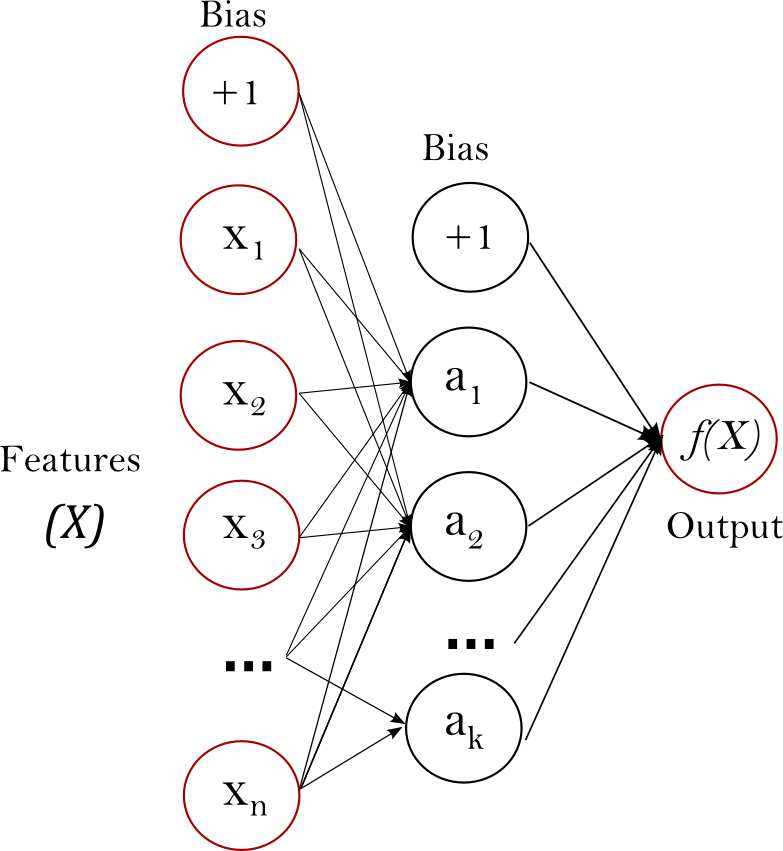
\includegraphics[width=7cm]{mlp-example.png}
                    \centering
                \end{figure}
                
                \paragraph{}Cada círculo na camada de entrada contém o que é chamado de neurônio $\{x_i|x_1,x_2,...,x_m\}$ e cada círculo da camada escondida representa um neurônio da camada escondida e transforma os valores da camada anterior baseado em uma soma com pesos $w_1x_1 + w_2x_2 + ... + w_mx_m$, seguido por uma função de ativação não linear $g(\cdot) : R \xrightarrow{} R$. A camada de saída recebe os valores da última camada escondida e transforma nos valores de saída \cite{mlp-model}.
                
            \subsection{Regressão Logística}
            
                \paragraph{}A regressão logística pode ser definida como uma técnica para calcular os parâmetros de um modelo logístico, ou seja, um modelo que se utiliza de funções logísticas para modelar o valor de uma variável binária dependente. Dessa maneira, essa técnica é vastamente utilizada para problemas de classificação cujas classes a serem previstas podem assumir 2 valores possíveis, como uma decisão de compra e não-compra de ações no mercado financeiro, escopo delimitado pelo projeto.
                
                \paragraph{}No modelo logístico, o logarítmo de acerto (referente à saídas classificadas como "1") é uma combinação linear de uma ou mais variáveis independentes binárias ou contínuas, que são as entradas do modelo. A probabilidade correspondente ao valor "1", pode variar continuamente entre 0 e 1 e a função que traduz essa probabilidade para a a classe final é chamada de função logística.
                
        \section{Técnicas de Validação}
        
            \paragraph{}Nessa seção são descritas as técnicas de validação usadas para o projeto.
            
            \subsection{Janelas Deslizantes}
            
                \paragraph{}Como o problema é de séries de tempo, a divisão do conjunto de dados entre treinamento e teste foi feita de modo que, obrigatoriamente, o conjunto de testes fosse composto por dados obtidos cronologicamente depois dos dados de treino. Dessa forma, foi possível obter previsões mais próximas do cenário real, em que a entrada do modelo obedece uma ordenação temporal.
                
                \paragraph{}Com o objetivo de obter o maior aproveitamento possível de dias utilizados para treino e previsão do conjunto de dados, foi utilizada a técnica de janelas deslizantes de treino e previsão. Nessa estratégia, utiliza-se um número $N$ de dias para formar o conjunto de treino e um número $N'$ para o conjunto de testes para realizar a validação. Na próxima iteração, utiliza-se o mesmo número de dias para as duas janelas, com a diferença que a janela de treino e de previsão tem início e fim do início e fim anteriores. A imagem \ref{img:sliding-validation} pode ser usada para ilustrar a explicação.
                
                
                \begin{figure}[h]\label{img:sliding-validation}
                    \caption{Janelas deslizantes com 4 dias usados para o conjunto de treino e 1 dia para o conjunto de teste}
                    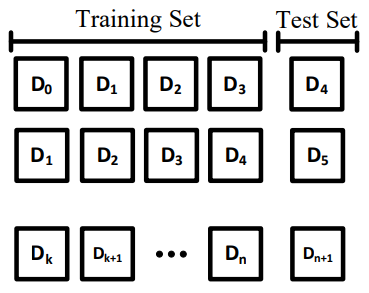
\includegraphics[width=8.3cm]{sliding-validation.PNG}
                    \centering
                \end{figure}
                
            \subsection{Expansão das Janelas Deslizantes}
            
                \paragraph{}Com o intuito de encontrar o número ótimo de dados de treino necessários para o modelo, foi feita uma iteração tal que, ao final do ciclo de janelas deslizantes de $N$ dias de treino, fosse iniciado um outro ciclo com $N+1$ dias para o conjunto de treino. Foi utilizada a linguagem de programação \textit{Python} para a implementação dessa lógica.
                
            \subsection{Parâmetros de validação}
            
                \paragraph{}Para cada previsão feita pelo modelo, cria-se uma matriz de confusão (\ref{img:matriz-confusao}) antes de extrair os parâmetros utilizados para mensurar a perfomance do modelo. 
                
                \begin{figure}[h]\label{img:matriz-confusao}
                    \caption{Matriz de confusão}
                    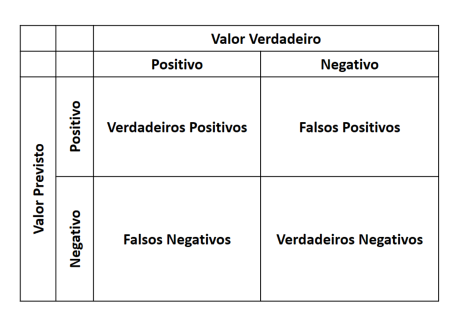
\includegraphics[width=10cm]{matrix-confusao.png}
                    \centering
                \end{figure}
                
                \paragraph{}Com a matriz de confusão, pode-se visualizar de forma mais direta os valores previstos em relação aos valores verdadeiros. Dessa forma, são de interesse para a performance do modelo o número de verdadeiros positivos e verdadeiros negativos em relação ao resto do conjunto.
                
                \paragraph{}Um verdadeiro positivo é quando uma classe classificada como "1" no conjunto de testes de fato possui o valor verdadeiro "1". Um falso positivo, por sua vez, refere-se a uma classe que é classificada como "1" enquanto possui "0" como valor verdadeiro. Pensamento análogo pode ser aplicado aos verdadeiros negativos e falsos negativos.
                
                \paragraph{}Para o domínio do trabalho, tem-se como interesse óbvio um modelo que seja capaz de obter mais acertos do que erros para obter lucro e, além disso, identifique o maior número possível de oportunidades de compra. A a matriz de confusão pode ser reaproveitada para gerar os parâmetros de validação abaixo.
                
                \subsubsection{Precisão}
                    \paragraph{}A precisão é definida como a quantidade de valores classificados corretamente como verdadeiros sobre a quantidade total de previsões verdadeiras do conjunto de teste. Pode ser calculada pela fórmula abaixo:
                    
                    \begin{equation}
                        P = \frac{VP}{VP + FP}
                    \end{equation}
                    
                    \paragraph{}Onde P é a precisão e VP e FP são classificadas como as amostras classificadas como verdadeiros positivos e falsos positivos, respectivamente.
                    
                \subsubsection{Revocação}
                    \paragraph{}A revocação é definida como a quantidade de valores classificados corretamente como verdadeiros sobre a quantidade total de verdadeiros do conjunto de teste. Pode ser calculada pela fórmula abaixo:
                    
                    \begin{equation}
                        R = \frac{VP}{VP + FN} = \frac{VP}{TP}
                    \end{equation}
                    
                    \paragraph{}Onde R é a revocação, FN é a quantidade de amostras classificadas como falso negativas e TP é o total de valores positivos do conjunto de teste.
                    
                \paragraph{}Para cada ciclo de uma determinada janela de treinamento, é calculada a média das precisões e das realocações obtidas de forma a obter a melhor combinação de dias de treino. Quanto mais alta a média das precisões, mais alta é a taxa de acerto obtida para futuras amostras. Se a realocação estiver alta, significa que o modelo está identificando grande parte das oportunidades de compra. Nesse ponto, é possível escolher a estratégia a ser seguida: manter um modelo mais seguro, que tenha menos sensibilidade para a hora de entrar no mercado, porém com maiores chances de acerto; manter um modelo que seja mais sensível para identificar oportunidades, porém menos preciso em sua previsão.
                
    \chapter{Resultados e Discussões}
    
        \paragraph{}Como estudo de caso para o projeto, foi escolhida a análise sobre a PETR4, ações preferências da Petrobrás, empresa voltou a ocupar em outubro de 2018 o título de mais valiosa do Brasil, chegando a bater a marca de R\$358 bilhões \cite{petr4-intro}. 
        
        \paragraph{}Para isso, foram importados todos os dados diários negociados da BM\&FBOVESPA de julho de 2018 até janeiro de 2019 e feito o pré-processamento descrito na seção \ref{sec:grouping}.
        
        \paragraph{}Após a importação dos dados brutos, escolheu-se empricamente uma janela de tempo de 3 minutos para a geração os indicadores de análise técnica com a saída determinada pela estratégia descrita na seção \ref{sec:estrategia-saida} para o intervalo futuro de tempo de um minuto a partir do tempo de fim da janela de tempo.
                
                
        

\chapter{Revisão Bibliográfica}

  Para ilustrar a completa adesão ao estilo de citações e listagem de
  referências bibliográficas, a Tabela \ref{tab:citation} apresenta citações de alguns dos trabalhos contidos na norma fornecida pela CPGP da
  COPPE, utilizando o estilo numérico.

  \begin{table}[h]
  \caption{Exemplos de citações utilizando o comando padrão
    \texttt{\textbackslash cite} do \LaTeX\ e
    o comando \texttt{\textbackslash citet},
    fornecido pelo pacote \texttt{natbib}.}
  \label{tab:citation}
  \centering
  {\footnotesize
  \begin{tabular}{|c|c|c|}
    \hline
    Tipo da Publicação & \verb|\cite| & \verb|\citet|\\
    \hline
    Livro & \cite{book-example} & \citet{book-example}\\
    Artigo & \cite{article-example} & \citet{article-example}\\
    Relatório & \cite{techreport-example} & \citet{techreport-example}\\
    Relatório & \cite{techreport-exampleIn} & \citet{techreport-exampleIn}\\
    Anais de Congresso & \cite{inproceedings-example} &
      \citet{inproceedings-example}\\
    Séries & \cite{incollection-example} & \citet{incollection-example}\\
    Em Livro & \cite{inbook-example} & \citet{inbook-example}\\
    Dissertação de mestrado & \cite{mastersthesis-example} &
      \citet{mastersthesis-example}\\
    Tese de doutorado & \cite{phdthesis-example} & \citet{phdthesis-example}\\
    \hline
  \end{tabular}}
  \end{table}
  
  É importante notar que, segundo a \href{http://www.poli.ufrj.br/graduacao_projeto.php}{Norma para a Elaboração Gráfica do Projeto de Graduação} da Escola Politécnica da UFRJ para trabalhos de conclusão de curso de engenharia de julho de 2012, as referências bibliográficas podem ser apresentadas de duas formas: $(i)$ Referências numeradas e $(ii)$ Referências em ordem alfabética. Para exibição numerada, em que a exibição das referências bibliográficas segue a ordem de citação usada no texto, use o comando \texttt{\textbackslash bibliographystyle\{coppe-unsrt\}}. Para exibição de referências bibliográficas em ordem alfabética, basta usar o comando \texttt{\textbackslash bibliographystyle\{coppe-plain\}} ao final do documento. 
  
  
  \chapter{Método Proposto}
  
  
  
  \chapter{Resultados e Discussões}
  
  
  
  \chapter{Conclusões}
  
  
  
  

  \backmatter
  \bibliographystyle{coppe-unsrt}
  \bibliography{example}

  \appendix
  \chapter{Algumas Demonstrações}
\end{document}
%% 
%%
%% End of file `example.tex'.
